\documentclass[../main.tex]{subfiles}

\begin{document}
    \textbf{Cztery fundamentalne działania }wspólne dla wszystkich procesów:
    \begin{itemize}
        \item \textbf{Specyfikowanie} oprogramowania
        \begin{itemize}
            \item zebranie wymagań,
            \item definiowanie funkcjonalności i ograniczeń dotyczących
            tworzonego software’u.
        \end{itemize}
        \item \textbf{Tworzenie} oprogramowania
        \item \textbf{Walidacja} oprogramowania
        \item \textbf{Ewolucja} oprogramowania
    \end{itemize}

    \hfill \\
    \textbf{Cykl życia systemu} - cały okres istnienia systemu:
    \begin{itemize}
        \item studium zastosowalności,
        \item analiza i specyfikacja,
        \item projektowanie i tworzenie,
        \item wdrażanie,
        \item pielęgnacja,
        \item aspekty usprawnienia.
    \end{itemize}

    \subsection{Modele procesu wytwarzania oprogramowania}
    \textbf{Model cyklu życia} systemu informatycznego ma na celu \underline{przedstawienie procesu} wytwarzania
    oprogramowania, który prowadzi do stworzenia działającego systemu.


    \subsubsection{Model kaskadowy}
    \begin{itemize}
        \item \textbf{wyizolowane etapy}, każdy musi być zakończony przed rozpoczęciem kolejnego
        \begin{itemize}
            \item \underline{Planowanie}: cele biznesowe, podstawowe wymagania, założenia, standardy, parametry,
            \item \underline{Analiza}: zdefiniowanie przeznaczenia systemu $\rightarrow$ kompletny, spójny i jednoznaczny model systemu,
            \item \underline{Projekt}: dekompozycja na podsystemy, wybór strategii budowania, projektowanie obiektów, wybór komponentów, opis interfejsów,
            \item \underline{Implementacja}: tworzenie kodu źródłowego, mapowanie modeli na kod,
            \item \underline{Testowanie}: znajdowanie różnic między rzeczywistym elementem a jego modelem,
            \item \underline{Pielęgnacja}.
        \end{itemize}
        \item Etapy podzielone na dwie części: \underline{twórczą} i \underline{weryfikacji}
        \item Ponowna praca, jeśli konieczna, jest wykonywana w kolejnych etapach - bardzo wysoki koszt błędów
        popełnionych we wstępnych etapach, adaptowanie zmian bardzo kosztowne.
        \item Koszty opracowania i akceptacji dokumentów są wysokie, powinien bvyć używany
        tylko jeśli wymagania są jasne i zrozumiałe.
        \item Marginalizacja roli klienta w procesie wytwarzania oprogramowania. Uzyskanie produktu zgodnego z wymaganiami
        silnie zależne od ich stabilności.
    \end{itemize}

    \subsubsection{Model V}
    \begin{figure}[H]
        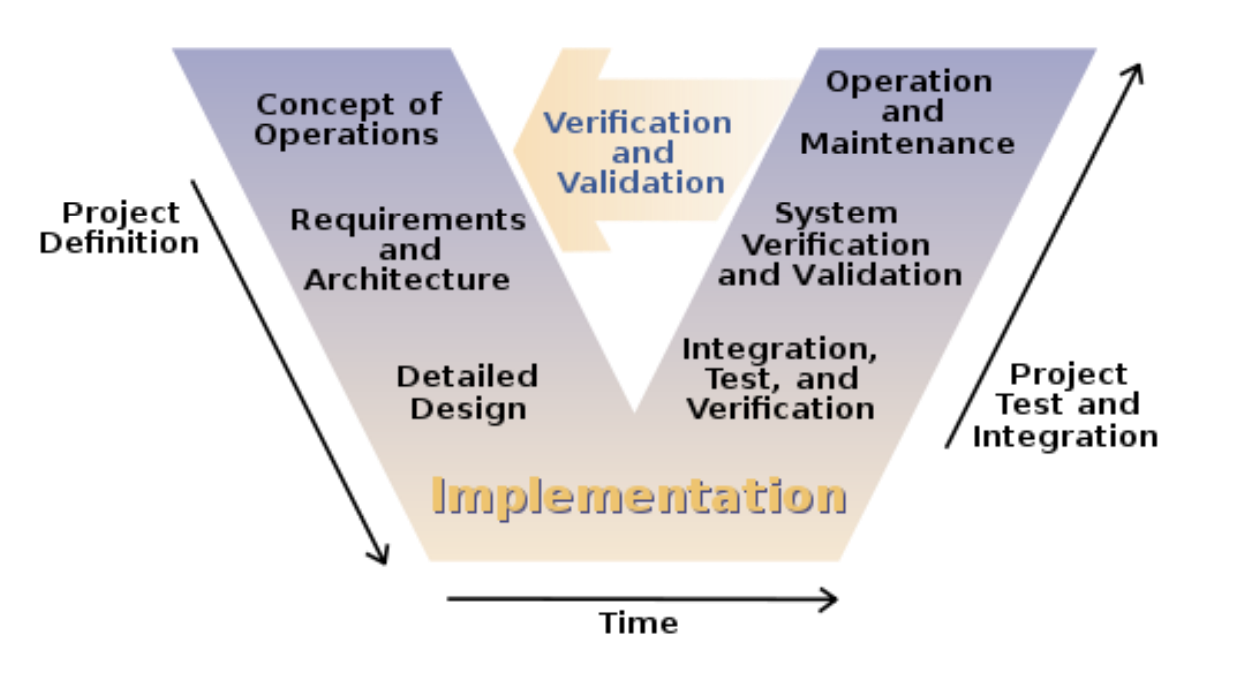
\includegraphics[width=\linewidth]{model_v.png}
    \end{figure}

    \subsubsection{Model Ewolucyjny}
    \begin{table}[H]
        \begin{center}
            \begin{tabular}{ p{8cm} c }
                \begin{itemize}
                    \item pozwala później określić wymagania do projektowanego systemu,
                    \item prototyp pomaga kształcić przyszłego użytkownika,
                    \item prototyp podnosi koszty w krótszej perspektywie, ale w
                    dłuższej może je obniżać,
                    \item zwykle prototyp jest wyrzucany.
                \end{itemize}
                &
                \raisebox{-\totalheight}{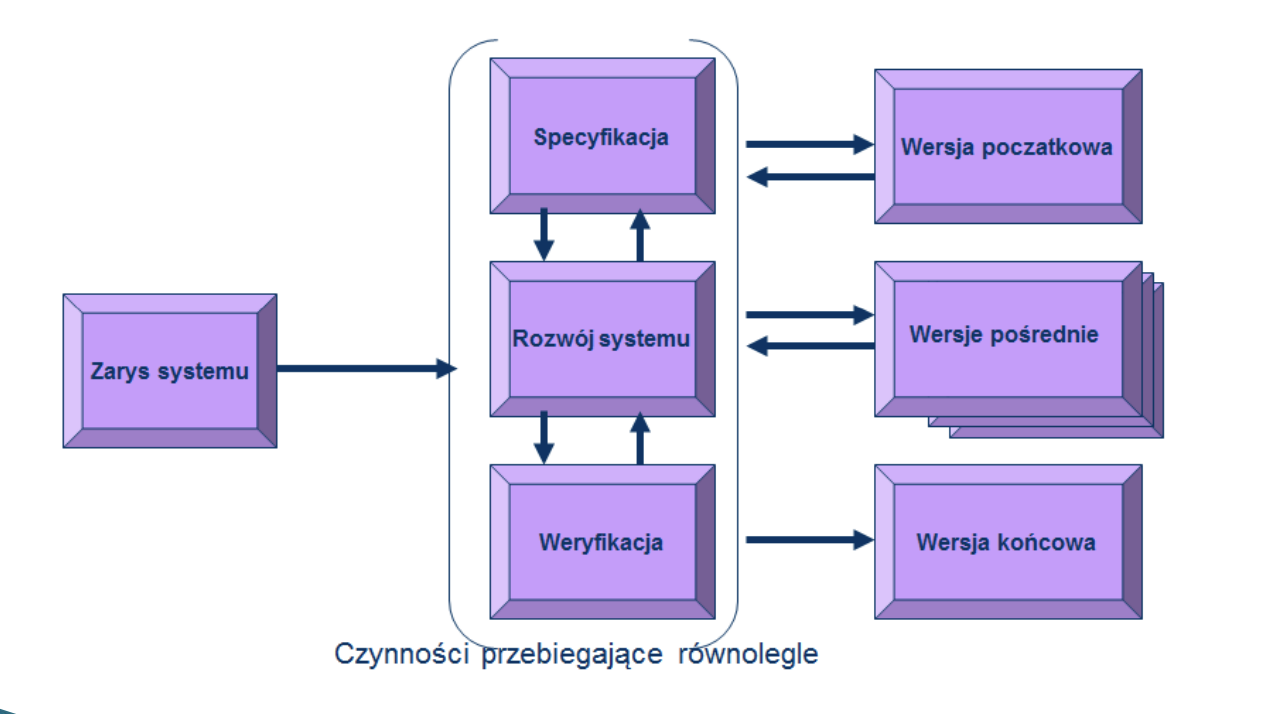
\includegraphics[width=0.5\textwidth]{model_ewolucyjny.png}}
                \\
            \end{tabular}
        \end{center}
    \end{table}


    \subsubsection{Model iteracyjny}

    \begin{table}[H]
        \begin{center}
            \begin{tabular}{ p{8cm} c }
                \begin{itemize}
                    \item pozwala na wczesne wykrywanie błędów,
                    \item łączy iteracje z klasycznym modelem kaskadowym,
                    \item łatwość wprowadzania zmian,
                    \item wymogi klienta dotyczące harmonogramu mogą utrudnić korzystanie z tego
                    modelu,
                    \item problemy z oszacowaniem ryzyka.
                \end{itemize}
                &
                \raisebox{-\totalheight}{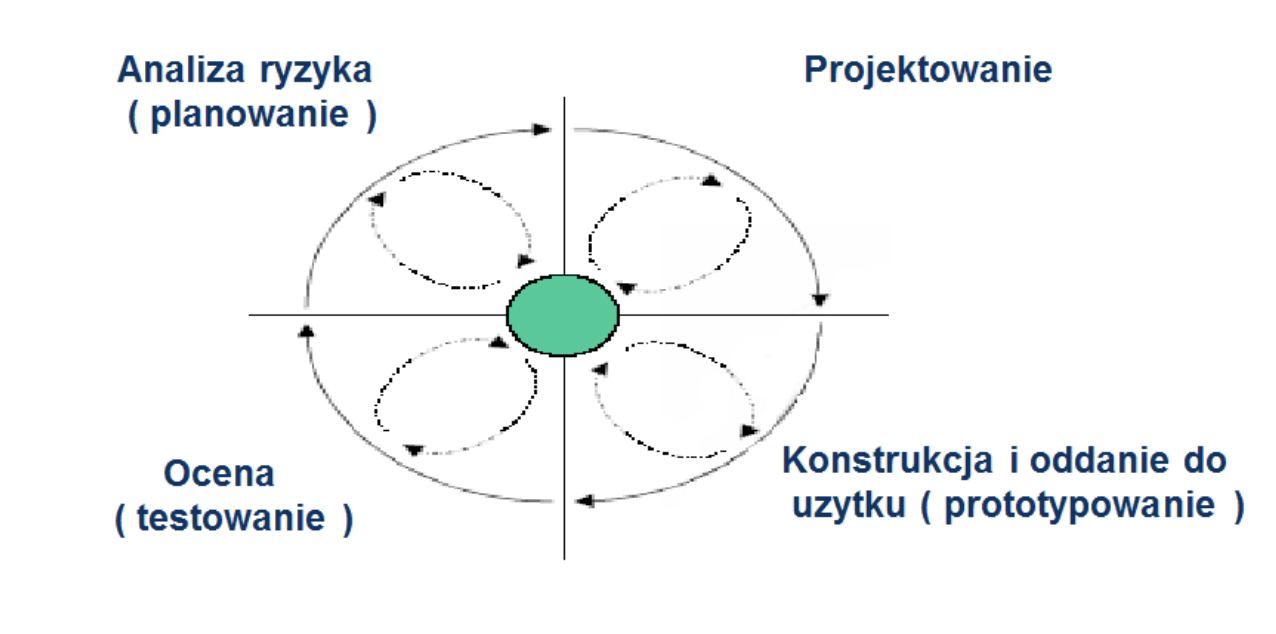
\includegraphics[width=0.5\textwidth]{model_iteracyjny.png}}
                \\
            \end{tabular}
        \end{center}
    \end{table}


    \subsubsection{Model spiralny}
    \begin{table}[H]
        \begin{center}
            \begin{tabular}{ p{8cm} c }
                \begin{itemize}
                    \item ciągłe monitorowanie i pomiar zmian,
                    \item zmiany poddawane są review użytkownika,
                    \item próba minimalizacji ryzyka niepowodzenia.
                \end{itemize}
                &
                \raisebox{-\totalheight}{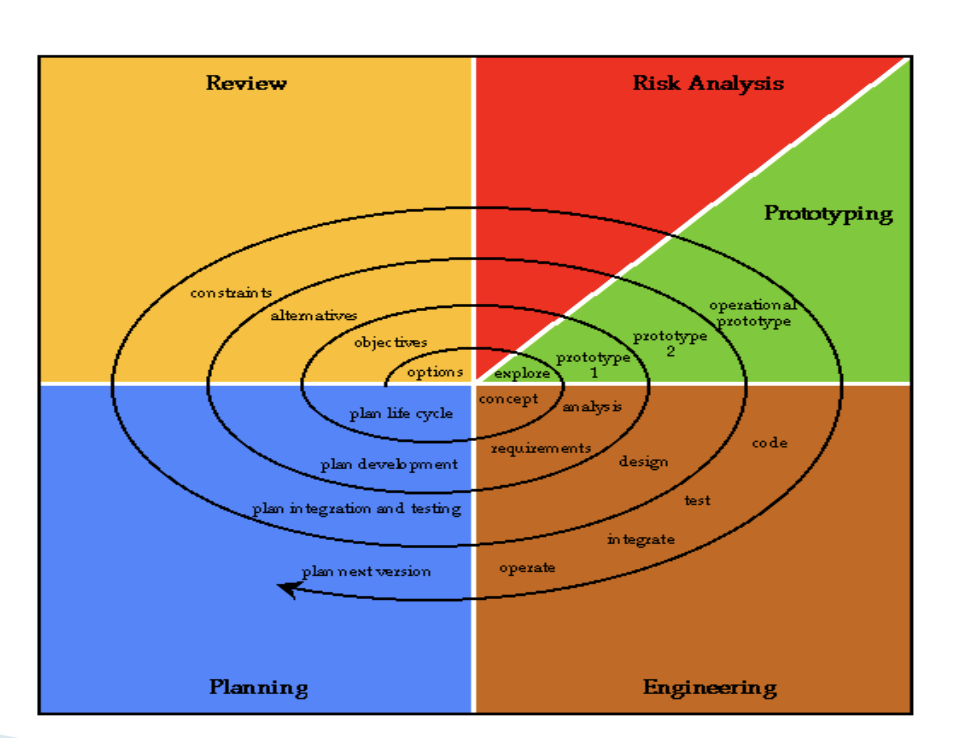
\includegraphics[width=0.5\textwidth]{model_spiralny.png}}
                \\
            \end{tabular}
        \end{center}
    \end{table}



\end{document}